\chapter{Random choise of target languages}


\section{Overview}

In this chapter we explore the effect of increasing number of target languages on the model performance in general.
Multiple possible outcomes can be expected at this experiment:
either performance drop due to the increased amount of languages to be processed by the model of the same size,
or the opposite - performance increase due to shared knowledge gained by the model from bigger and varying dataset. 
Also, either of these options can be true for different target languages in different scale.

First of all, performance drop is expected. Considering that the size of the model is fixed, so is its capacity. At some moment adding more target languages should lead to the decrease in translation quality for each of every target language


\section{Performance drop on massively multilingual setup}
1-to-3, 5, 7, etc. models on en-to-36 dataset (0.9 mil. sentences per target language)

When the size of the model is fixed, adding more translation directions usually causes
worsening of its performance. Multiple studies have shown this to be truth for
many-to-many setup.

In \cite{aharoni-etal-2019-massively} models with up to 103 languages were tested.
English centric in-house dataset was used to train En\to{}Any and Any\to{}En multilingual models.
The average number of examples per language pair is 940k:
for 13 out of the 102 pairs there were less than one million examples available.
All languages from 5-to-5 model are present in 25-to-25, same is true for all languages from 25-to-25 with respect to 50-to-50 and so forth.
In all cases they trained large Transformer model with 473.7M parameters.
As can be seen on Table \ref{tab:aharoni-2019-performance-drop}, the quality of translation
is significantly worse when model is trained to translate more languages.
However, it is worth reminding that this many-to-many experiment may have different reasons due to many-to-one direction present in it.

The decrease of model's performance with adding more target langueges
is clearly shown in \cite{aharoni-etal-2019-massively}.


\begin{table}[h!]
\centering
\begin{tabular}{r|cccc}
\toprule
           & En-Ar & En-Fr & En-Ru & En-Uk \\
\midrule
5-to-5     & \textbf{12.42} & \textbf{37.3} & \textbf{24.86} &         16.48  \\
25-to-25   &         11.77  &         36.79 &         23.24  & \textbf{17.17} \\
50-to-50   &         11.65  &         35.83 &         21.95  &         15.32  \\
75-to-75   &         10.69  &         34.35 &         20.7   &         14.59  \\
103-to-103 &         10.25  &         34.42 &         19.9   &         13.89  \\
\bottomrule
\end{tabular}
\mycaption{BLEU scores for translation in one direction
        (part of Table 7 from \citep{aharoni-etal-2019-massively})
	}{
		Model trained on 5-to-5 English centric dataset 
		(English to any and any to English) scores 12.42 BLEU for
		English-Arabic test set. Every language from 5 languages
		of 5-to-5 data set is included into 25-to-25 set, as well
		as every language from 25-to-25 data set is included into
		50-to-50 and so forth.
	}
\label{tab:aharoni-2019-performance-drop}
\end{table}


\begin{figure}[h]
	\begin{minipage}{0.48\textwidth}
	\centering
	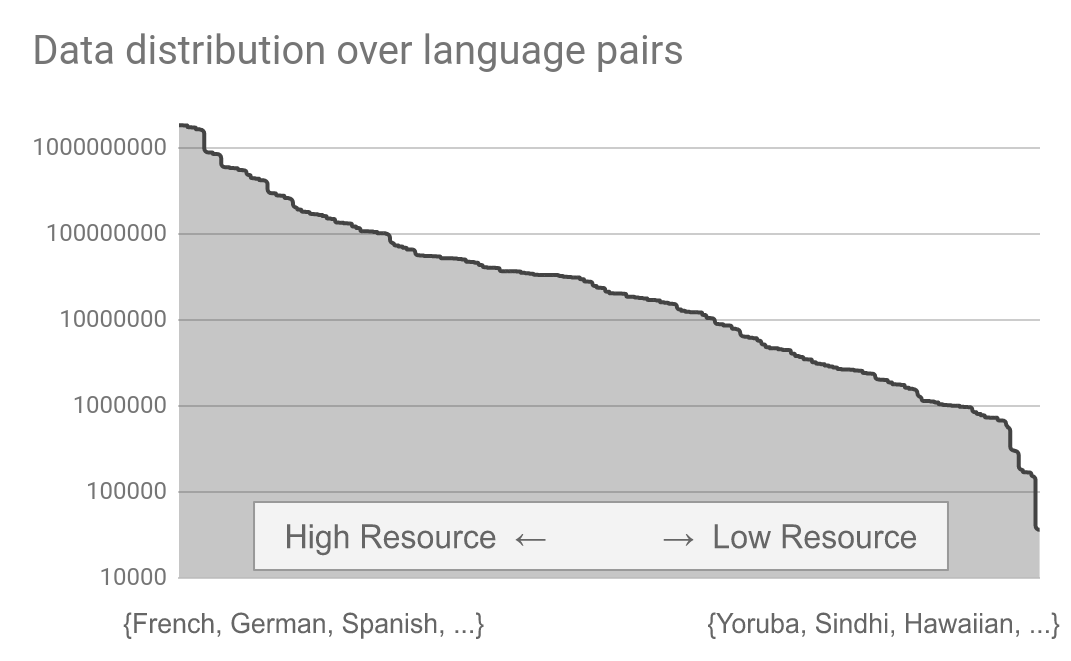
\includegraphics[width=0.9\columnwidth]{../img/arivazhagan-2019-data-distribution.png}
	\end{minipage}\hfill
	%\vspace*{\floatsep}% https://tex.stackexchange.com/q/26521/5764
	\begin{minipage}{0.48\textwidth}
	\centering
	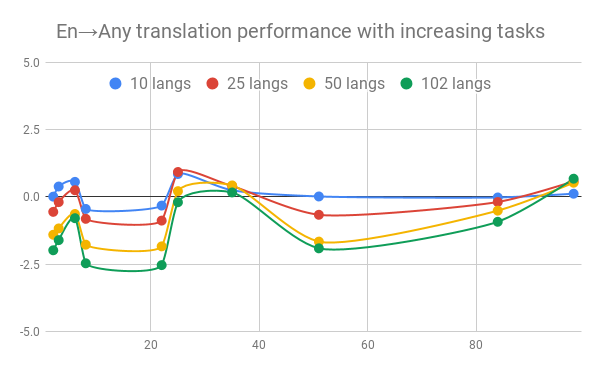
\includegraphics[width=0.9\columnwidth]{../img/arivazhagan-2019-diff-per-n-targets.png}
	\end{minipage}
	\mycaption{
		Tranlsation performance for 102 languages from 
		\citet{arivazhagan-2019-mmnmt-in-the-wild}
	}{
		Axis \emph{X} is shared between left and right plot.
		On axis \emph{X} there are languages sorted by amount of training data.
		Left: amount of training data (axis \emph{Y}) for a language.
		Right (best viewed in color): Effect of increasing the number of languages on
		the translation quality. On the axis \emph{X} the languages are sorted the 
		same way as on the left plot. The points visualized are 10 languages
		that are present in all setups
		from En $\leftrightarrow$ 10 to En $\leftrightarrow$ 102.
	}
	\label{fig:arivazhagan-2019-diff-per-n-targets}
\end{figure}


\begin{table}[h!]
\begin{subtable}[t]{0.45\linewidth}
	\centering
	\begin{tabular}{rrrr}
	\toprule
	n\_targets &   mean &   std & count \\
	\midrule
	         1 &  41.40 &  ---  &   1 \\
	         2 &  40.60 &  0.20 &   3 \\
	         3 &  39.39 &  0.62 &   8 \\
	         4 &  39.40 &  0.71 &   2 \\
	         5 &  38.45 &  0.52 &   6 \\
	\bottomrule
	\end{tabular}

	\caption{
		En\to{}Bg for \emph{Europarl/v7} dataset.
		}
	\label{tab:bg/Europarl/v7}
\end{subtable}
\begin{subtable}[t]{0.45\linewidth}
	\centering
	\begin{tabular}{rrrrrrr}
	\toprule
	n\_targets & mean & count & std \\
	\midrule
	        1 &     19.50 &    1 &   --  \\
	        2 &     18.88 &    4 &  0.39 \\
	        3 &     17.45 &    4 &  0.52 \\
	        4 &     17.80 &    2 &  0.42 \\
	\bottomrule
	\end{tabular}
	
	\caption{
		En\to{}Ru for \emph{OpenSubtitles/v2016} dataset.
		}
	\label{ table:ru/OpenSubtitles/v2016 }
\end{subtable}
\mycaption{BLEU score change with adding target languages}{
    (a) First row: for mono-lingual En\to{}Bg model test BLEU score is 41.40.
    Second row: for 3 (column \emph{count}) En\to{}Any
    models with two target languages
    (column \emph{n\_targets}) one of which is Bulgarian
    the mean BLEU score is 40.60 with standard deviation 0.20.
    (b): same way as (a)
}
\end{table}



% \begin{table}[h]
% \centering
% \begin{tabular}{rrrrrrr}
% \toprule
% n\_targets & mean & count & std \\
% \midrule
%         1 &     --.-- &    1 &    -  \\
%         2 &     18.86 &    8 &  0.31 \\
%         3 &     17.59 &    8 &  0.48 \\
%         4 &     17.80 &    4 &  0.35 \\
% \bottomrule
% \end{tabular}
% 
% \caption{
% 	BLEU score for En\to{}Ru translation on test set part of
% 	\emph{OpenSubtitles/v2016} dataset.
% 	Description is the same as for table \ref{tab:bg/Europarl/v7}
% 	}
% \label{ table:ru/OpenSubtitles/v2016 }
% \end{table}

\section{Performance decrease on richer data sets}
1 to 3, 4, 5 on UN corpus (much more sentence pairs per target language)
\cite{eisele-chen-2010-multiun}


